\section{Berechnungen}
Wir haben Berechnungen gemacht, um eines besseres Übersicht von die nötige Energie der dieses Projekt angefragt.
Hier sind nur die Hauptergebnisse angezeigt; alle Berechnungen befinden sich \href{https://github.com/accefa/doku/tree/master/bin/Berechnungen.xlsx}{hier}. \\ \\
Mit der Benutzung und Umwandlung von die schräger Wurf Formeln, könnten wir die nötige Geschwindigkeit ausrechnen und damit die notwendige Energie.
\begin{figure}[h!]
	\centering
	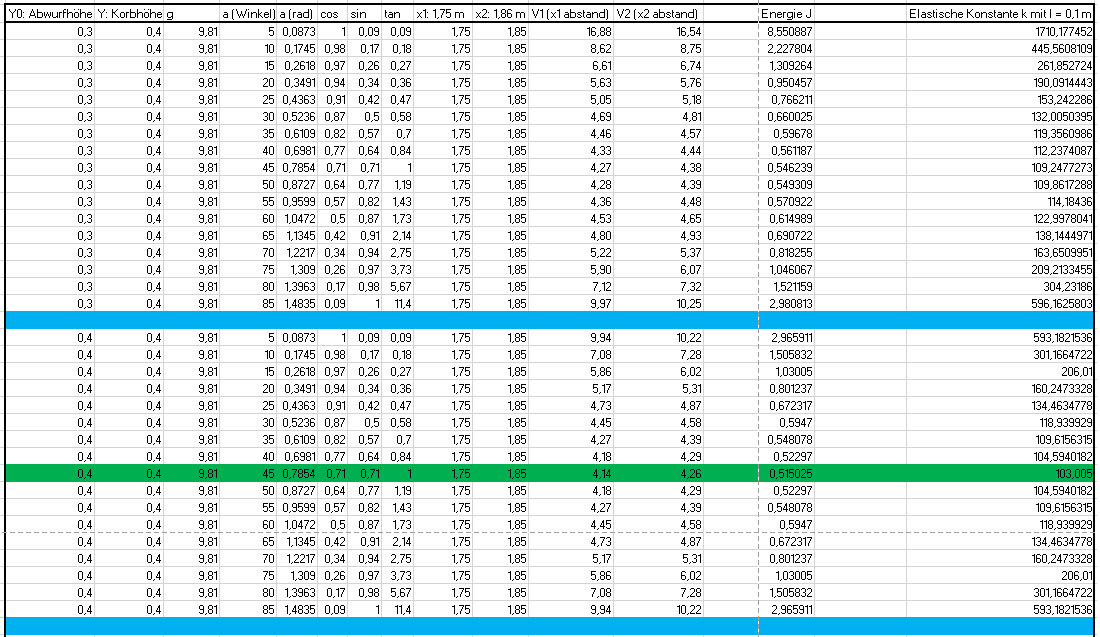
\includegraphics[width=1\textwidth]{../../fig/Geschwindigkeit_und_eleastische_Konstante.png}
	\caption{Berechnungen von die Abwurfgeschwindigkeit und nötige Federkonstante}
	\label{fig:Berechnungen von die Geschwindigkeit}
\end{figure}
\newpage
Um eine Idee von die nötige Leistung der unseres Motor braucht, haben wir berechnet das Trägheitsmoment der Ball und vom stossende Stab, und mit die vorherige berechnete nötige Geschwindigkeit, könnten wir die Drehzahl und Drehmoment der Motor berechnen.
\begin{figure}[h!]
	\centering
	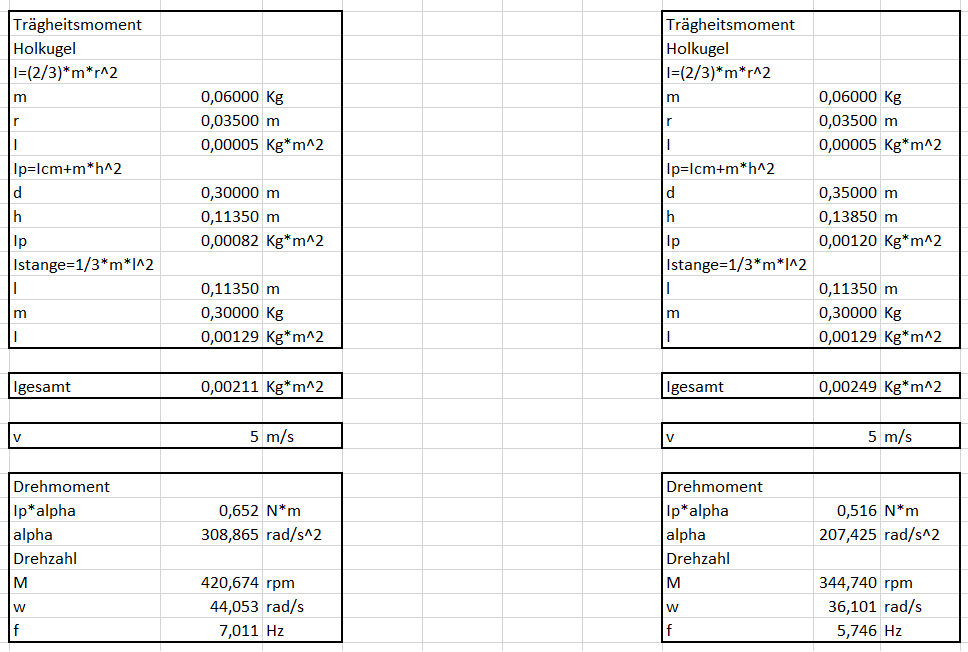
\includegraphics[width=1\textwidth]{../../fig/Berechnungen_Propeller.png}
	\caption{Berechnungen für die Notwendige Drehzahl und Drehmoment vom Motor für Konzept 1:Propeller}
	\label{fig:Berechnungen für der Propellerkonzept}
\end{figure}
